% !TEX encoding = UTF-8 Unicode

\documentclass[10pt]{article}

%%
%% Packages
%%
\usepackage[english]{babel}
\usepackage[utf8]{inputenc}
\usepackage{pifont}
\usepackage{enumerate}
\usepackage{amssymb,amsfonts,amsopn,amscd}
\usepackage{ifthen}
\usepackage{epsfig}
\usepackage{color}
\usepackage{amsmath}
\usepackage{booktabs}
\usepackage{colortbl}
\usepackage{subfig}
\usepackage{natbib}
\usepackage[colorlinks]{hyperref}
\usepackage{verbatim}

\newtheorem{remark}{Remark}[section]

%% Mise en page
\textwidth=16.0cm
\textheight=24cm
\topmargin=-2cm
\addtolength\oddsidemargin{-2cm}
\addtolength\evensidemargin{-2cm}
\renewcommand{\baselinestretch}{1.0}

%% Macros collaboratives
\definecolor{mygreen}{rgb}{0.0,0.6,0.0}
\newcommand{\tbd}[1]{{\bfseries \textcolor{cyan}{[TODO: #1]}}}
\newcommand{\discuter}[1]{{\bfseries \textcolor{mygreen}{[DISCUTER: #1]}}}
\newcommand{\mjtop}[1]{{\bfseries \textcolor{blue}{[MJ2P: #1]}}}
\newcommand{\ptomj}[1]{{\bfseries \textcolor{magenta}{[P2MJ: #1]}}}
\newcommand{\avantapres}[2]{\textcolor{red}{[{\bfseries AVANT}: #1]}\textcolor{blue}{[{\bfseries APRES}: #2]}}

%% Document properties
\title{{\bfseries From print to web to e-paper...}\\A design-centric approach for the reinvention of newspaper}
\author{Pierre Kornprobst}
\date{May 2019}

%% Document starts
\begin{document}
\maketitle

\section{Context: The future is (also) the past}

The digital era has completely transformed the newspaper industry which is still struggling for finding the best revenue models, stretched between printed and online news.
As print ad revenue cratered, the need to squeeze revenue from digital sources grew and pushed publishers to invest on developing online news content, again making up the money in advertising.

Online news offer a number of advantages and interesting characteristics to the users such as, e.g.,  continuous updates, the possibility of searching, intuitive navigation,  hyperlinks, and of course the possibility to read news mostly everywhere with any portable device. 
However, the quality gap between online news and printed newspaper remains very large. 
This is due to two main reasons.

The first reason is technical and related to the fact that website should be legible on any platform. This is made thanks to responsive web design principles, allowing the layout to respond to the user behavior and environment based on platform, screen size, and orientation.
However, making sites that can refactor themselves for small screens implies a strong simplifications in the structure of informations.
Websites mostly present news in a linear fashion, thus missing the editorial organization found in printed newspapers.

The second is directly related to the ad revenue model that pushed news websites to their breaking point.
There is a situation now where ads, even on reputable sites, occupy an important portion of the pages (see example in Figs.~\ref{fig:imaone}--\ref{fig:imatwo}). 
Some professional in the field even wonder if the journalists still matter about how to  deliver news to human beings or instead how many advertisements are served.
\begin{figure}[htbp]
\centerline{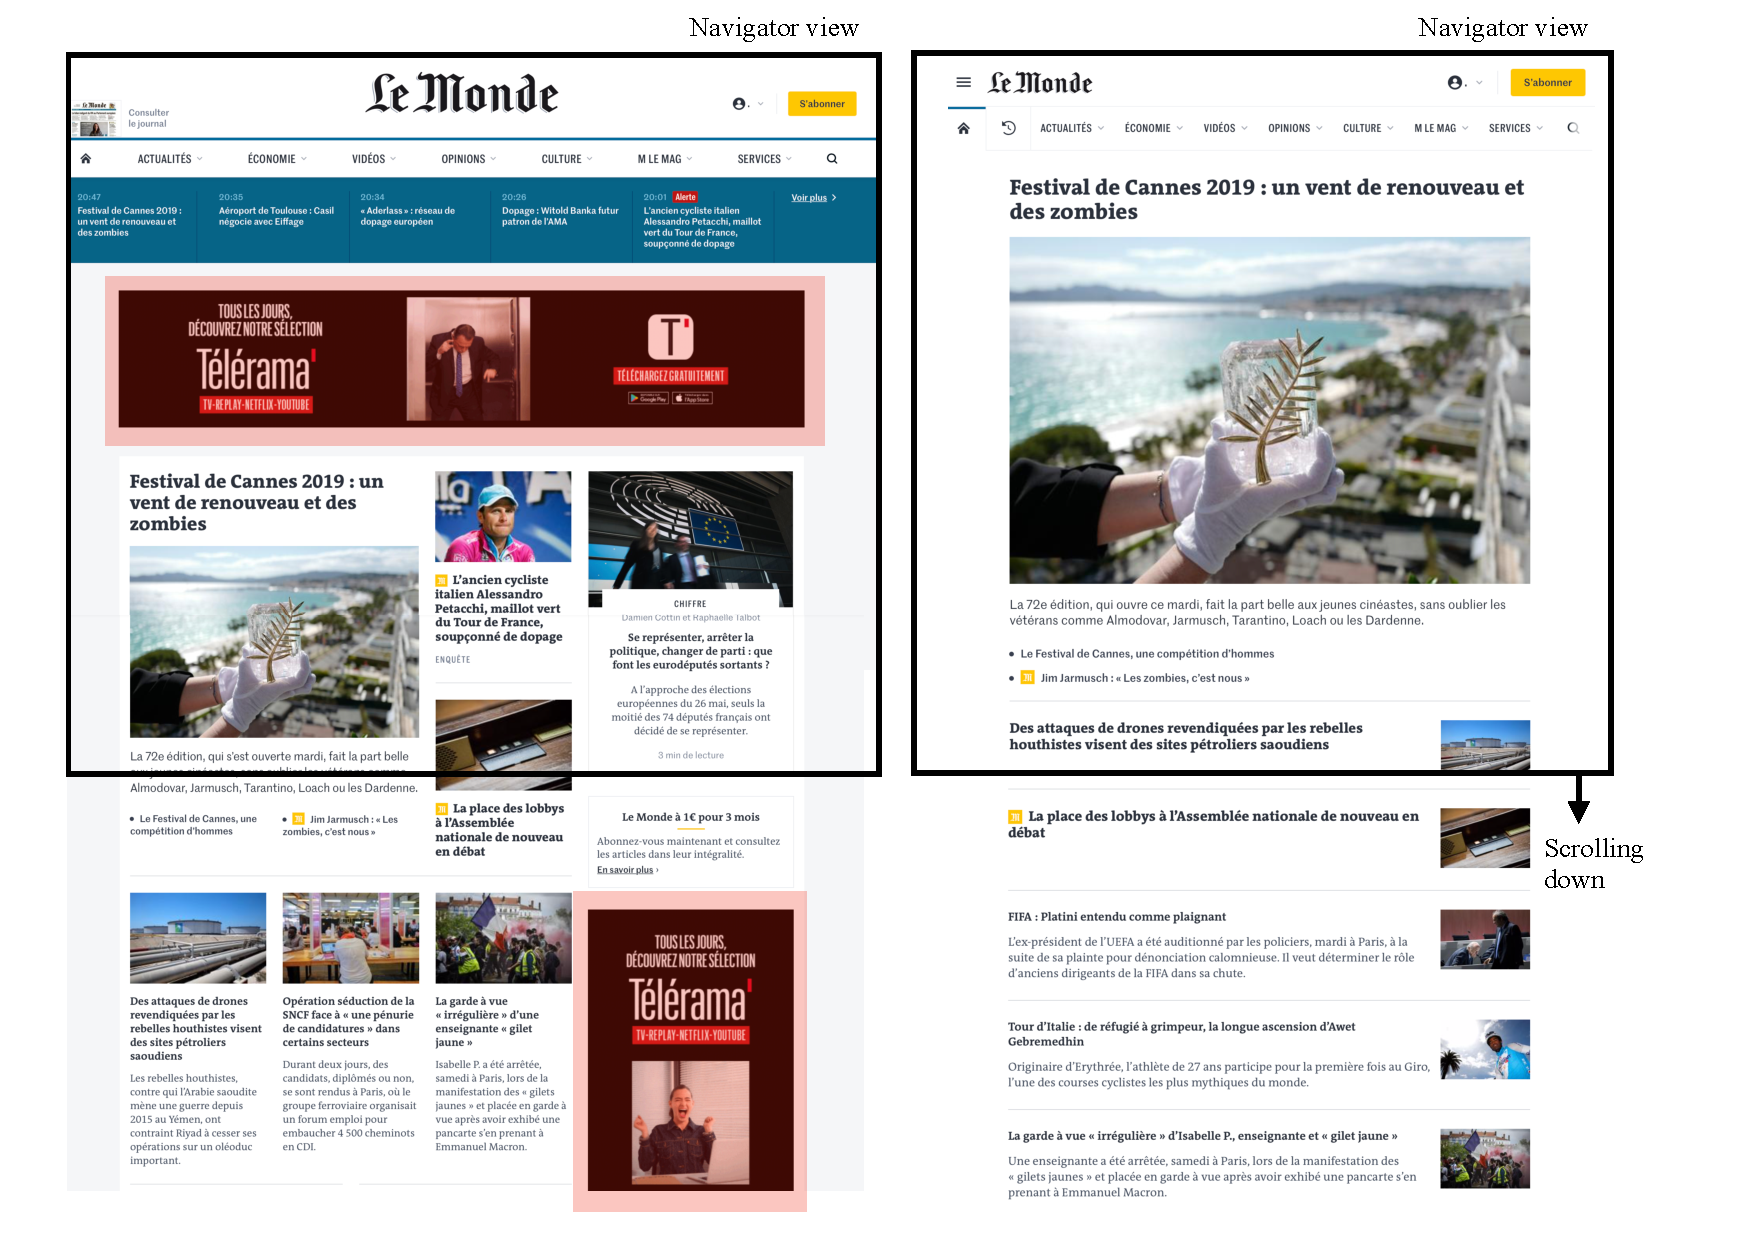
\includegraphics[width=\textwidth]{ima/lemonde-online1}}
\caption{\label{fig:imaone}Illustration of responsive design principle from Le Monde website. Changing slightly the width of the navigator may completely change the layout of the page, from a column organization to a very linear one. The content is accessible via scrolling. The presence of ads (highlighted in red) occupies a very important place in the display. Note that these ads from the front page are changing at every reload of the page, thus also creating some instability in the presentation of the content.}
\ \\
\centerline{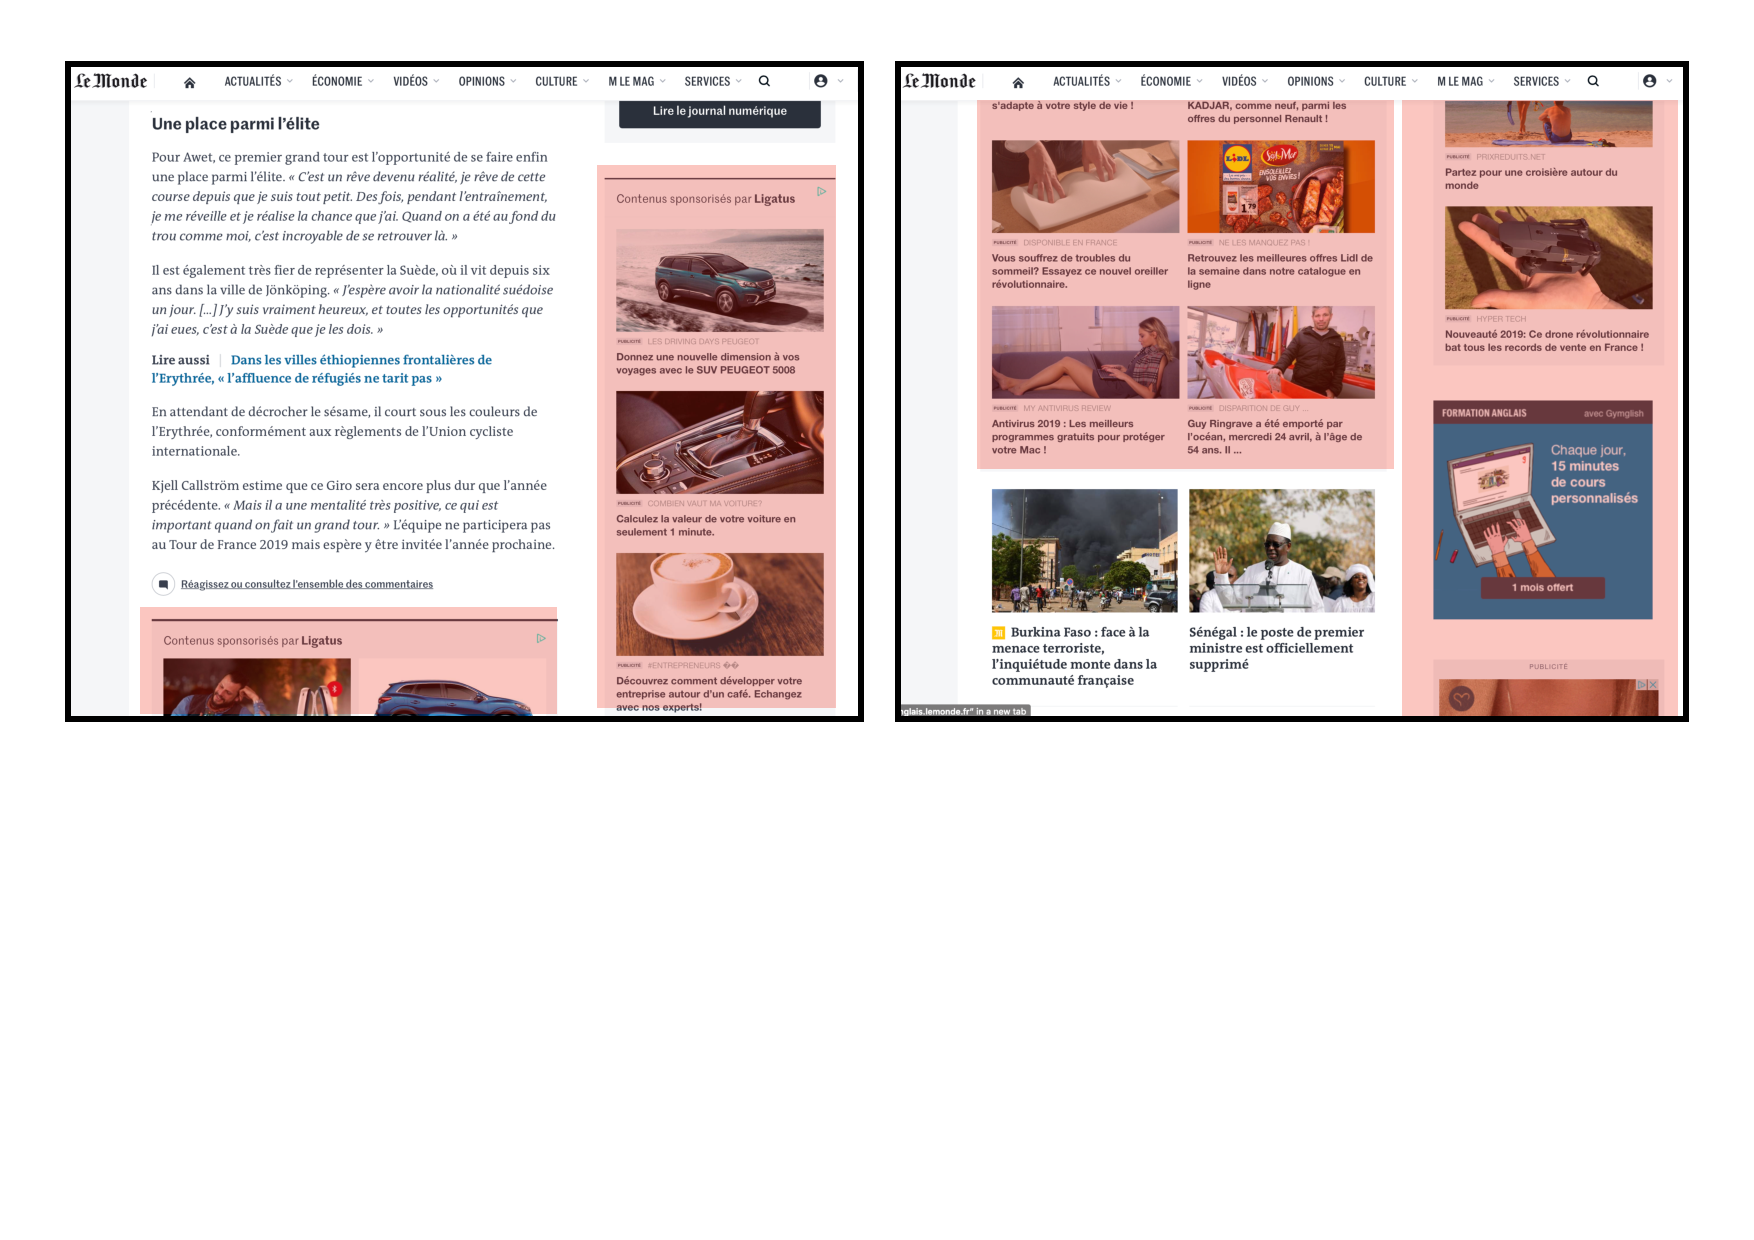
\includegraphics[width=\textwidth]{ima/lemonde-online2}}
\caption{\label{fig:imatwo}Illustration of ads for a given article: Ads are highlighted in red, showing their impact on the design. Not only they can occupy a large portion of screen but also there positioning may introduce confusion between what is content and what is ads (see right-hand side figure).}
\end{figure}

\begin{quote}
"{\itshape Ads are just brutal for what they do to your browser and sort of utter lack of regard they have for user experience}", 
Ian Adelman, Chief Creative Officer at New York Magazine
\end{quote}

Interestingly, not only this revenue model raises questions in terms of user experience, but also its future is not guaranteed due to Google and Facebook's dominance of the digital advertising market. 
New revenue models are experimented by some actors (e.g., digital subscription, membership models) but more importantly, what needs to be invented is a new way to consume news which focuses on user experience.

This naturally brings us back to print newspapers for which user experience is a central point.
Indeed, despite its decline, print newspapers continue to be an indispensable point of reference in terms of quality. 
By quality, here we refer to newspaper design, that is having a strong, consistent and appealing visual approach to enhance the impact and comprehension of a story.

\begin{quote}
"{\itshape To design an newspaper means to organize the information in such a way that it will facilitate the makeup of the issue [...] and in the end, to convey the information to the reader in the clearest way possible}",
from~\cite{vignellivignelli:07}
\end{quote}

This quest of beautiful design is not a cult of "art for art's sake" advocated by a few extreme visual experts. Neither it is just about making things look good using proper grids, type, color, and visuals. Newspaper design is about user experience and engagement of the readers.

\begin{quote}
"{\itshape The link between audience engagement and good design has never been stronger and it's becoming even more crucial to commercial success in the digital era.}",
From~\cite{morell:16}. 
\end{quote}

In light of all this, the business and design of news are inextricably linked and should not be considered as different goals. 
Achieving a stronger engagement of the audience is the key and focusing on design is a necessity.  
As such, we believe that print newspapers have a future in the digital age and will continue to play a key role within news production. 
Online news are one option which has been already developed, providing several interesting characteristics, but showing its limitations in terms of user experience.
Our ambition if to develop a new type of news distribution through electronic paper (e-paper) targeting the best of the two words, bringing a comfortable reading experience enriched by characteristics from the digital world to better serve the audience. 




\section{State-of-the-art: Leverage e-paper as replacement for the print newspaper?}

Amongst the variety of display technologies, we are interested the E-ink technology which is a popular type of electronic paper (e-paper).
Several eReaders using this technology are currently available on the the market (e.g., the Barnes and Noble nook, Sony Reader, Amazon Kindle or BOOX). 
Their main advantage is that they give the same reading experience as on paper (such as high contrast and the possibility to read in sunlight).
The electronically made print also enables e-paper the same viewing angles as printed material because it is a reflecting display technology in contrast to projecting technologies such as LCD screens.
These tablets are thin and can be large (e.g., 13.3" for BOOX MAX2).
Another advantage of the technology is the low power consumption (power is only needed when the display is updated). 
Some current limitations are related to color, multimedia and interactivity are not well supported in some eReaders.
However, taken together, these properties make e-paper technology especially suitable for content traditionally offered in print such as newspapers, books, and magazines. 

%%%% CITE ALSO BELOW
%Screen and Paper Reading Research – A Literature Review
%https://www.tandfonline.com/doi/full/10.1080/00048623.2016.1227661
%Australian Academic & Research Libraries 
%Volume 47, 2016 - Issue 3
%Screen and Paper Reading Research – A Literature Review
%Pages 160-173 
%Gemma Walsh

In the litterature, one finds several papers comparing reading experience on-screen versus print versions~\cite{hollander-krugman-etal:11,walsh:16,neijens-voorveld:18}. More specifically, in~\cite{hollander-krugman-etal:11} the authors have studied if readers of a print newspaper behave would consider e-reader(in this case, the Kindle DX)  a good substitute from the print edition. Interestingly, all participants to this study confirmed the pleasure of using e-paper device for its portability, simplicity, clarity, legibility and readability but they also raised  concerns about the order and manner in how the device presented the news.
Indeed, unlike the newspaper print edition in which a story’s significance is signaled by its size and placement on a page, stories on the Kindle equal in size and as a list with no obvious priority as to their significance. This lack of editorial organization left may participants unsatisfied with e-paper, because of several consequences on the user experience, navigation and serendipity. Their feedback confirm the important of design and storytelling: the story you want to tell is as important as the way in which they are told. 
\begin{quote}
"{\itshape I couldn’t get the big picture of anything}"\\
"{\itshape I don’t know who decides what article is most important}"\\
"{\itshape Kindle gives you no way to kind of see how the newspaper evaluated the importance of the story}"\\
"{\itshape It's not visually very interesting}"\\
"{\itshape I really like being surprised by -- when I’m looking at the hard copy -- finding an article that I wouldn’t normally gravitate to, but because of the picture or something, you read it, and you kind of feel enriched because it’s something that you wouldn’t ordinarily read}"
\end{quote}

So, from a user experience perspective, the optimal future e-newspaper should combine the portability, readability and overview from the printed newspaper with the possibilities of online media such as constant updates, interactivity and personalization, offering a high quality news reading experience anytime and anywhere~\cite{ihlstrom-eriksson-etal:04}. From a business perspective, new revenue models have also been proposed and could be a source of inspiration~\cite{ihlstrom-kalling-etal:08,akesson:09}.




%%%%% ENTER
%%%%% ihlstrom-kalling-etal:08
%See paper 5, page 146: BUSINESS MODELS FOR M-SERVICES: EXPLORING THE E-NEWSPAPER CASE FROM A CONSUMER VIEW
%@article{article,
%author = {Ihlstr{\"o}m Eriksson, Carina and Kalling, Thomas and \AA kesson, Maria and Fredberg, Tobias},
%year = {2008},
%month = {01},
%pages = {29-57},
%title = {Business Models for M-Services: Exploring the E-Newspaper Case from a Consumer View.},
%volume = {6},
%journal = {JECO}
%}

%%%%% ENTER
%%%%% akesson:09
%Report
%Gothenburg Studies in Informatics, Report 42, September 2009
%ISSN 1400-741X (print), ISSN 1651-8225 (online), ISBN 978-91-628-7877-1 http://hdl.handle.net/2077/20887
%DIGITAL INNOVATION IN THE VALUE NETWORKS OF NEWSPAPERS
%Maria Åkesson



%% Bibliography
% \renewcommand{\refname}{Nouveau nom}
\bibliographystyle{plain}
% Version en ligne (apres montage de smb://sop-nas2b/www-sop-tools)
%\bibliography{/Volumes/www-sop-tools/biblio/bibfiles/odyssee/odyssee}
%\bibliography{odyssee}
% Version locale (l'updater via svn si besoin)
\bibliography{bib}

\end{document}



